\subsection{Движение по орбите}
\begin{figure}[t]
	\centering
	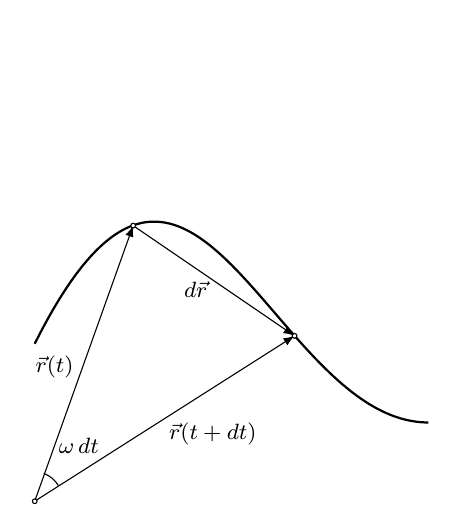
\begin{tikzpicture}
		\footnotesize
		
		%	\foreach \x in {0, .1,...,5} {
		%		\draw [line width=.1pt] (\x, -3) -- (\x, 3);
		%	};
		%
		%	\foreach \y in {-3, -2.9,...,3} {
		%		\draw [line width=.1pt] (0, \y) -- (5, \y);
		%	};
		
		\draw [thick] (0, 0) .. controls (2, 4) and (3, -1) .. (5, -1);
		\draw [-latex] (0, -2) -- (1.25, 1.5);
		\draw [-latex] (0, -2) -- (3.3, .1);
		\draw [-latex] (1.25, 1.5) -- (3.3, .1);
		
		\draw (.3, -1.8) arc(31:70:0.36);
		
		\draw (.6, -.3) node [anchor = east] {$\vec{r}(t)$};
		\draw (1.6, -.9) node [anchor = north west] {$\vec{r}(t + dt)$};
		\draw (2.3, 0.9) node [anchor = north east] {$d\vec{r}$};
		\draw (0.2, -1.5) node [anchor = south west] {$\boldsymbol{\omega} \,dt$};
		
		\draw[fill=white] (1.25, 1.5) circle (0.03);
		\draw[fill=white] (3.3, .1) circle (0.03);
		\draw[fill=white] (0, -2) circle (0.03);
		
	\end{tikzpicture}
	\caption{}
\end{figure}

Рассмотрим такую физическую величину, как \term{секториальная скорость}~--- это векторная величина, описывающая ориентированную площадь, заметаемую радиус вектором тела за единицу времени. Пусть в момент времени $t$ тело находилось в точке $\vec{r}(t)$, а через промежуток времени $dt$~--- в точке $\vec{r}(t + dt)$. Обозначим перемещение тела за этот промежуток времени как $d\vec{r}$. Его можно выразить через скорость тела в момент времени $t$, считая ее постоянной на промежутке от $t$ до $t + dt$: $d\vec{r} = \vec{v} \, dt$. Площадь, которую заметает радиус-вектор тело $\vec{r}(t)$ равна половине параллелограмма, построенного на векторах $\vec{r}(t)$ и $d\vec{r}$. Поэтому можно записать
\begin{equation*}
	\vec{s} = \frac{1}{2} [\vec{r} \times \vec{v} dt],
\end{equation*}
следовательно секториальная скорость равна
\begin{equation*}
	\boldsymbol{\sigma} = \frac{d \vec{s}}{dt} = \frac{1}{2} [\vec{r} \times \vec{v}] = \frac{\vec{l}}{2} = \frac{\vec{L}}{2m},
\end{equation*}
где $\vec{l}$~--- удельный момент импульса (на единицу массы). Полученное выражение доказывает \imp{второй закон Кеплера}.

С другой стороны, перемещение $d\vec{r}$ можно выразить через угловую скорость $\boldsymbol{\omega}$, как $d \vec{r} = [\vec{r} \times \boldsymbol{\omega}\,dt]$. Тогда
\begin{equation*}
	\boldsymbol{\sigma}
	= \frac{1}{2} \big[ \vec{r} \times [\vec{r} \times \boldsymbol{\omega} ]\big]
	= \frac{1}{2} \left(\vec{r} \underbrace{(\vec{r}, \boldsymbol{\omega})}_0 - \boldsymbol{\omega} ( \vec{r}, \vec{r} ) \right)
	= \frac{r^2 \boldsymbol{\omega}}{2}.
\end{equation*}

Получим еще одно важное соотношение~--- \term{интеграл энергии}~--- формулу для скорости тела на орбите с большой полуосью $a$ в точке, удалённой на расстояние~$r$ от центрального тела с массой $M$. Для этого рассмотрим  сначала точку перицентра ($q$, <<п>>) и апоцентра ($Q$, <<a>>) данной орбиты, запишем для них закон сохранения энергии и закон сохранения момента импульса:
\begin{gather*}
	-\frac{GMm}{q} + \frac{m v^2_\text{п}}{2} = -\frac{GMm}{Q} + \frac{m v^2_\text{а}}{2},\\
	mv_\text{п}q = mv_\text{a}Q.
\end{gather*}
Из ЗСМИ и выражений для перицентрического~$q$ и апоцентрического~$Q$ расстояний через большую полуось $a$ и эксцентриситет $e$ имеем:
\begin{equation*}
	\frac{v_\text{а}}{v_\text{п}} = \frac{1 - e}{1 + e}.
\end{equation*}
Использую это соотношения, преобразуем ЗСЭ:
\begin{gather}
	\frac{v_\text{п}^2}{2} \left( 1 - \frac{(1 -e)^2}{(1 + e)^2} \right) = GM \left( \frac{1}{a(1-e)} - \frac{1}{a(1+e)} \right),\\
	\frac{v_\text{п}^2}{2} \cdot \frac{ 1 + 2e + e^2 - 1 + 2e - e^2}{(1+e)^2} = \frac{GM}{a} \cdot \frac{1 + e - 1 +  e}{(1+e)(1-e)},\\
	v_\text{п} = \sqrt{\frac{GM}{a}}\sqrt{\frac{1+e}{1-e}}, \quad \quad v_\text{a} = \sqrt{\frac{GM}{a}}\sqrt{\frac{1-e}{1+e}}.
\end{gather}
Запишем теперь ЗСЭ для перицентра и произвольной точки орбиты на расстоянии $r$:
\begin{gather*}
	-\frac{GMm}{q} + \frac{m v^2_\text{п}}{2} = -\frac{GMm}{r} + \frac{m v^2}{2},\\
	-\frac{GMm}{q} + \frac{GMm}{2a} \cdot \frac{1+e}{1-e} = -\frac{GMm}{r} + \frac{m v^2}{2},\\
	v^2 = GM \left( \frac{2}{r} - \frac{2}{a(1 - e)} + \frac{1+e}{a (1-e) }\right) = GM \left( \frac{2}{r} - \frac{1}{a} \right),
\end{gather*}
\begin{equation}
	v = \sqrt{ GM \left( \frac{2}{r} - \frac{1}{a} \right)}.
	\label{eq:int-energy}
\end{equation}
Полученное выражение и называется интегралом энергии. Согласно \eqref{eq:int-energy} и \eqref{eq:ellipse-pol-eq} для скорости тела в произвольной точке орбиты также справедливо выражение
\begin{equation}
	v = \sqrt{\frac{GM}{p}\cdot(1 + 2 e \cos \nu + e^2)},
\end{equation}
где $\nu$~--- истинная аномалия, а $p$~--- фокальный параметр.

Найдем величину момента импульса пробной массы $m$ на эллиптической орбите. В силу постоянства данной величины, можно выбрать любую точку орбиты для её поиска. Проще всего рассмотреть перицентр или апоцентр, рассмотрим первый.
\begin{multline*}
	L
	= m v_q q
	= m \sqrt{\frac{GM}{a} \frac{1+e}{1-e}} \cdot a(1-e) =\\
	= m \sqrt{GMa (1 + e)(1-e)}
	= m \sqrt{GMa(1-e^2)}
	= m \sqrt{GMp}.
\end{multline*}

Для параболической также рассмотрим точку перицентра:
\begin{multline*}
	L
	= m v_q q
	= m v_2(q) q
	= m \sqrt{\frac{2GM}{q}} \cdot q =\\
	= m \sqrt{2GMq}
	= m \sqrt{2GM \cdot \frac{p}{2}}
	= m \sqrt{GMp}.
\end{multline*}

